\subsection{Filter}

Wie schon im Kapitel technische Grundlagen werden die Filter gebraucht um harmonische Oberwellen heraus zu filtern. Im Projektauftrag [x] wird definiert, dass Oberwellen ab 5kHz nicht mehr im Signal erwünscht sind. Darum müssen Oberwellen die eine höhere Frequenz haben, unterdrückt werden damit diesen nicht die Messung verfälschen.

\begin{minipage}[h]{0.5\textwidth} 
\begin{figure}[H]
\begin{center}
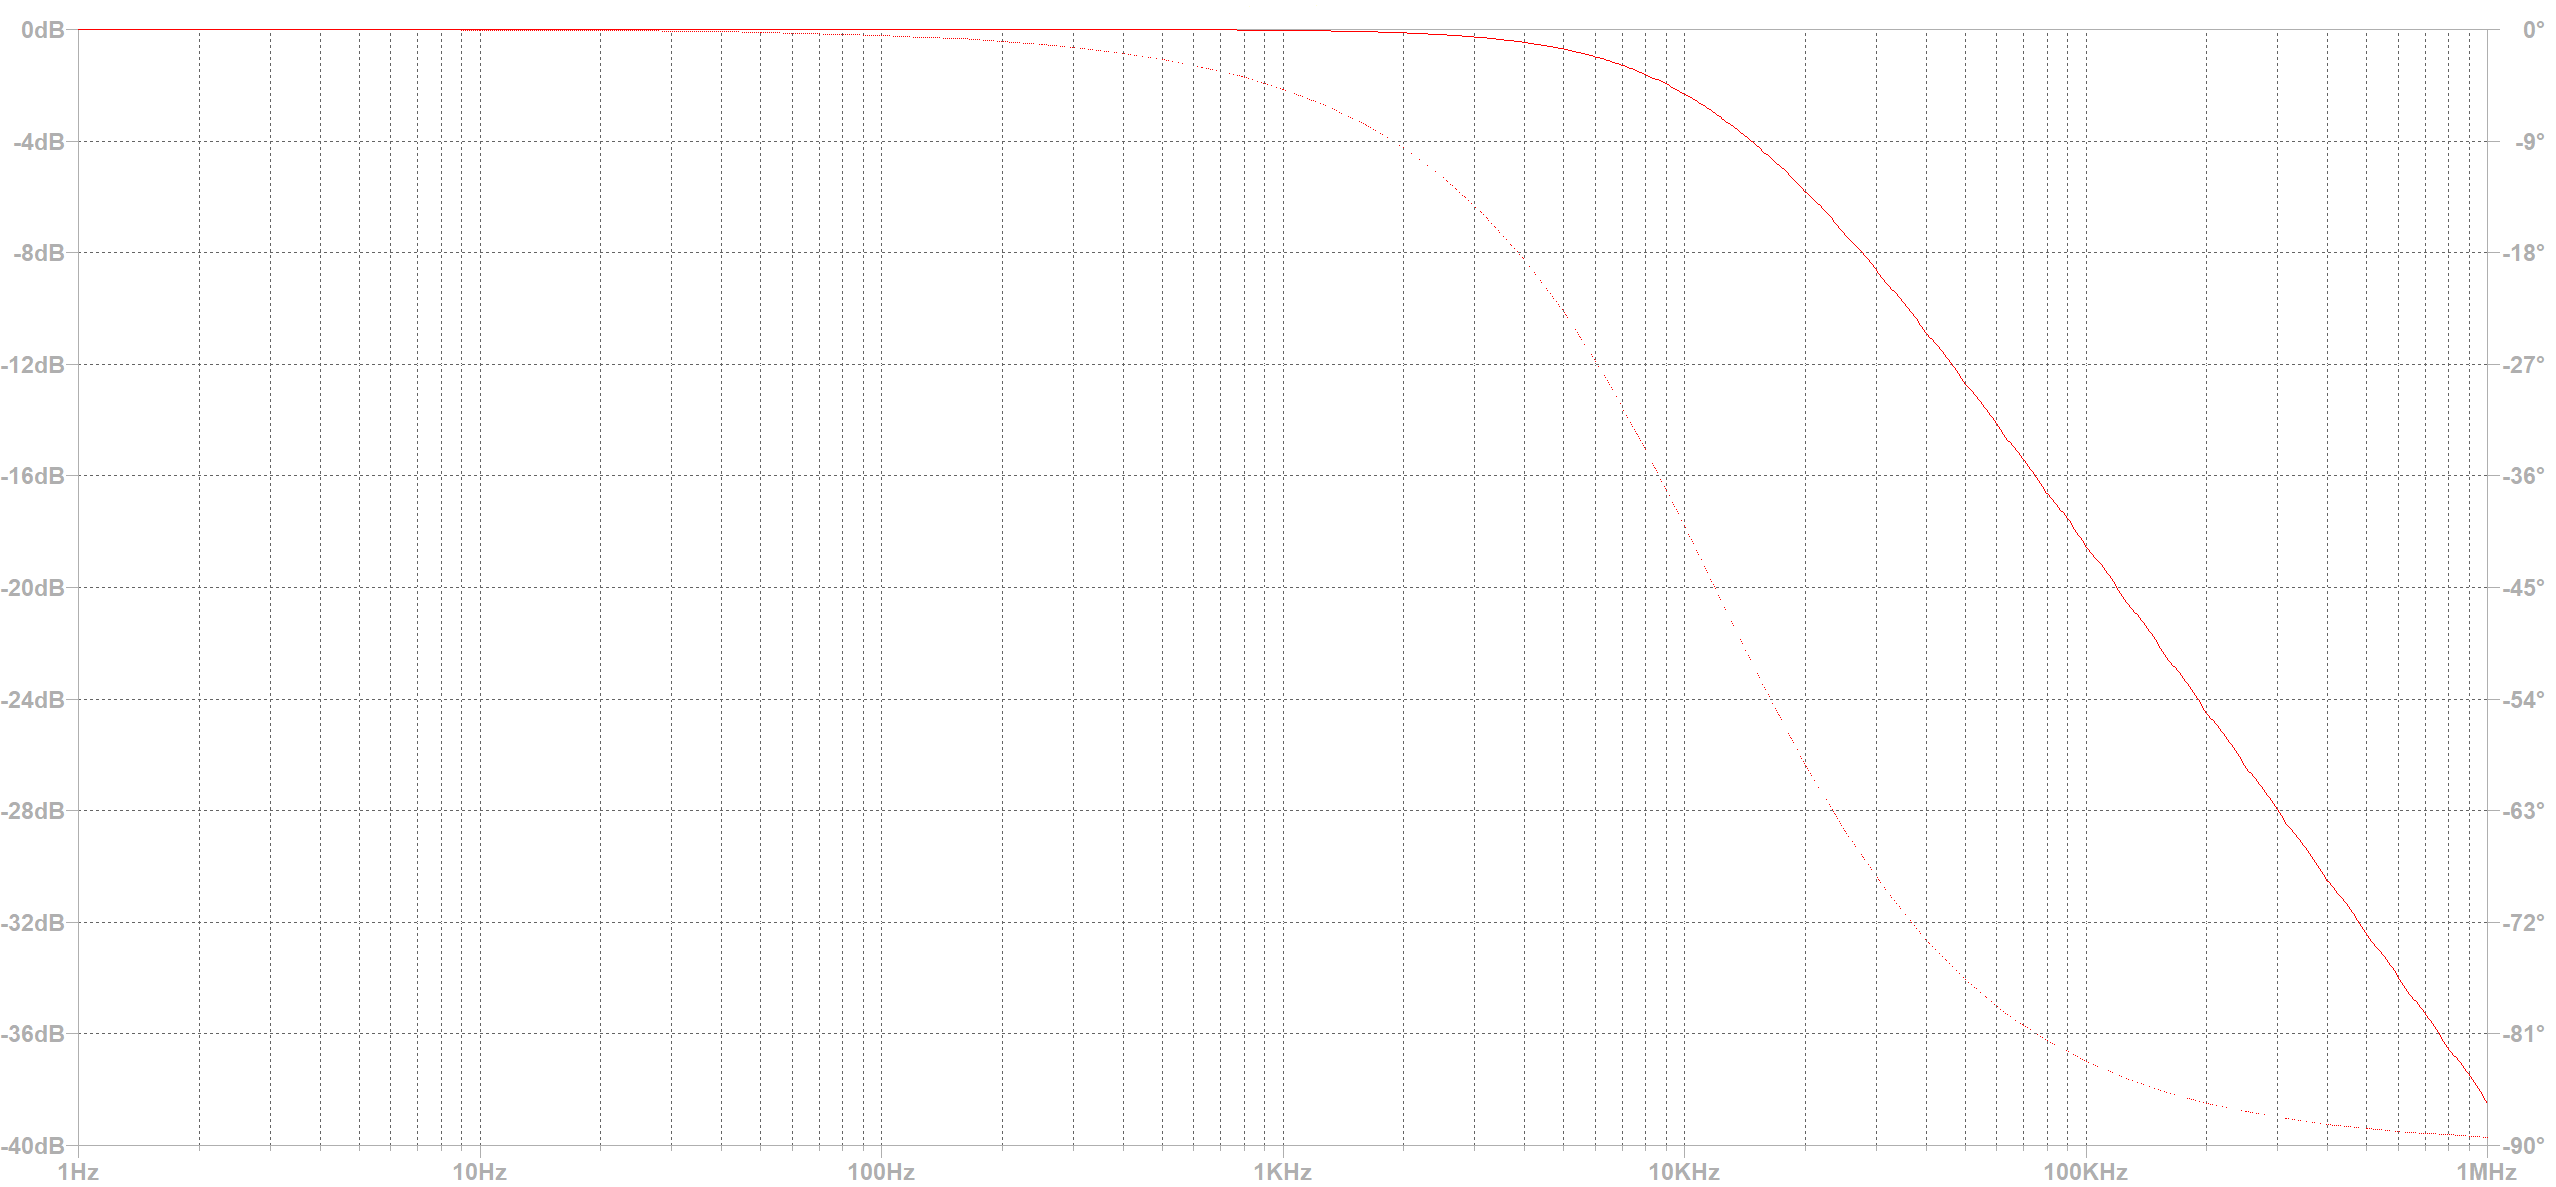
\includegraphics[width=0.9\textwidth]{images/Analoge_Schaltung_Frequenzgang.png}
\caption{Frequenzgang Tiefpass-Filter 1. Ordnung}
\end{center}
\end{figure}
\end{minipage}
\begin{minipage}[h]{0.5\textwidth}
Für das Projekt sind Tiefpass-Filter nötig die höhere Frequenzen unterdrücken und tiefe Frequenzen passieren lassen. Auf dem nebenstehenden Bild ist ein typischer Frequenzgang eines Tiefpass-Filters 1.Ordnung zu sehen. Da für das Projekt die Signale auch verstärkt werden müssen, sind Aktive-Filter naheliegend.[x]
\end{minipage}


\subsubsection*{Dimensionierung}

\begin{minipage}[h]{0.5\textwidth}
Die Wahl fiel auf Butterworth-Filter mit Sallen/Key-Topologie 2. Ordnung. Diese bietet den Vorteil, dass sie nicht invertierend ist. Dadurch ist ein Operationsverstärker ausreichend pro Signalpfad. Die Butterworth-Koeffizienten bringen den Vorteil, dass sie flach sind im Durchlassbereich und einen relativ eckigen Übergang bieten.[x] Jedoch wurde überlesen, dass mit dieser Filtertopologie nur Verstärkungen bis $A=3$ realisierbar sind. Bei höheren Verstärkungen können die instabil werden. 
\end{minipage}
\begin{minipage}[h]{0.5\textwidth} 
\begin{figure}[H]
\begin{center}
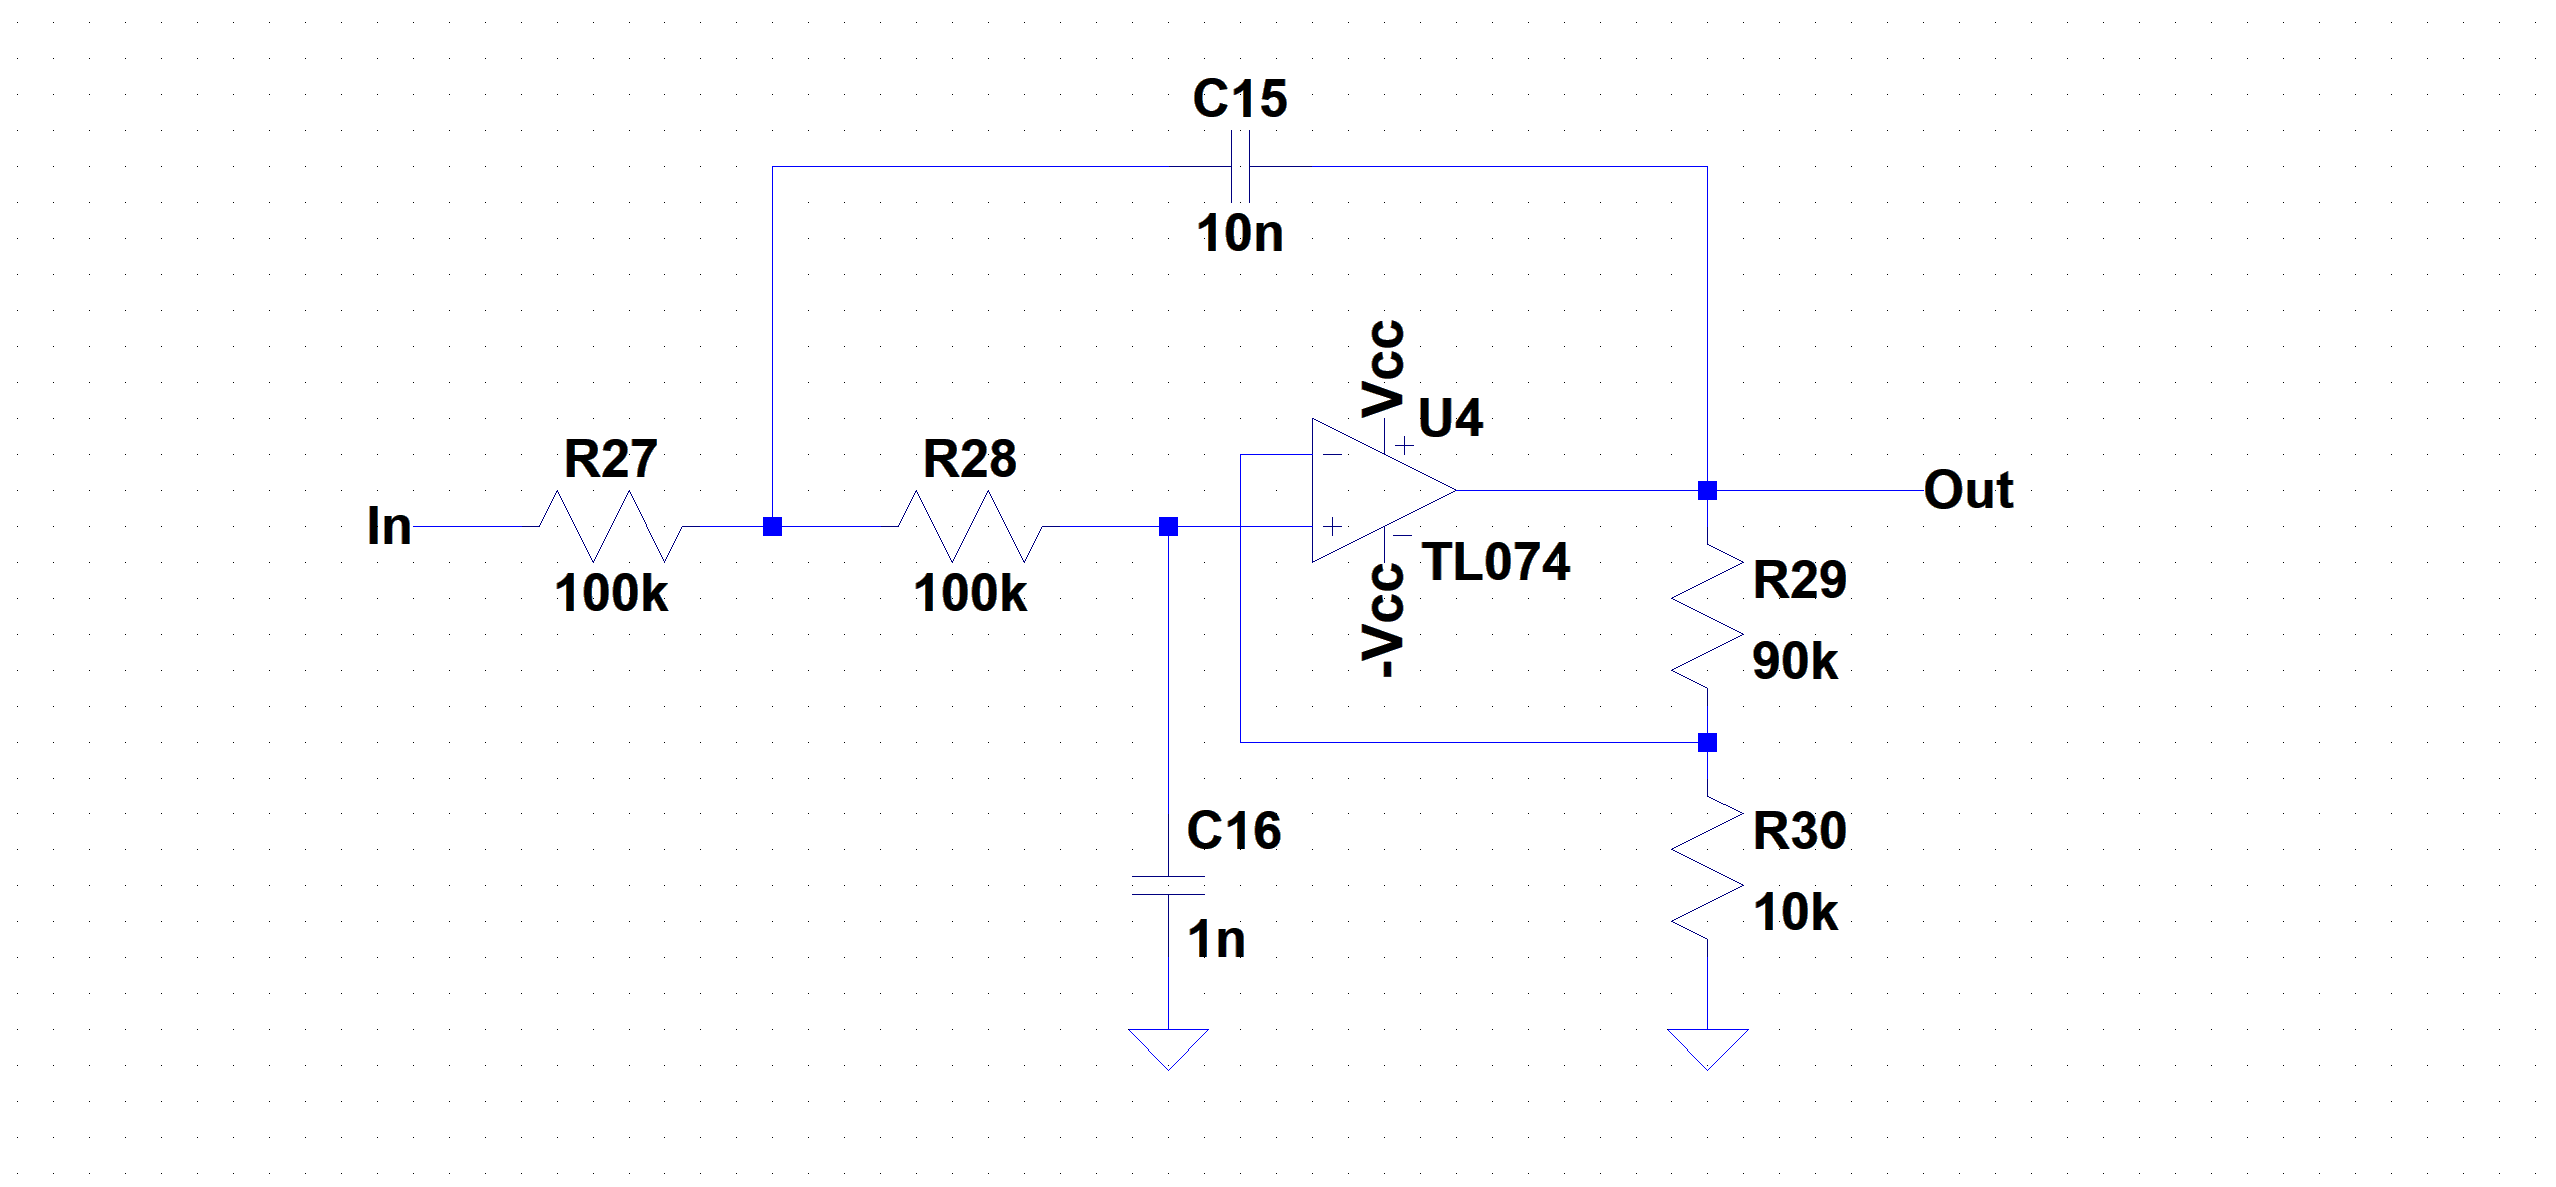
\includegraphics[width=0.9\textwidth]{images/Analoge_Schaltung_Sallen.png}
\caption{Sallen/Key-Topologie Tiefpass-Filter 2. Ordnung}
\end{center}
\end{figure}
\end{minipage}


\subsubsection*{Realisierte Filter}
Zuerst wurden die Sallen/Key-Filter realisiert. An den Operations-Verstärker wurden praktisch keine Anforderungen gestellt. Er soll ein GWP[x] von mindestens 800k besitzen und nicht Rail-to-Rail sein. Dadurch wurde einer verwendet der an Lager war. Dies ist der TL074, der praktischerweise 4 Operations-Verstärker in einem Gehäuse vereint. Die passiven Bauteile wurden mithilfe einer Formel[x] aus dem Internet erstellt, die sich im laufe des Projektes als falsch herausstellte.

\begin{minipage}[h]{0.5\textwidth}
Nachdem der Print gefertigt war, waren die Filter instabil wegen den zu grossen Verstärkungen. Aus der Not wurden die Filter umgebaut in einen passiven Filter 1.Ordnung und ein nachfolgende Verstärkung. Dafür musste nur der Kondensator C15 entlötet werden, damit ein Unterbruch entsteht und für den R27 wurde eine Drahtbrücke eingelötet.
\end{minipage}
\begin{minipage}[h]{0.5\textwidth} 
\begin{figure}[H]
\begin{center}
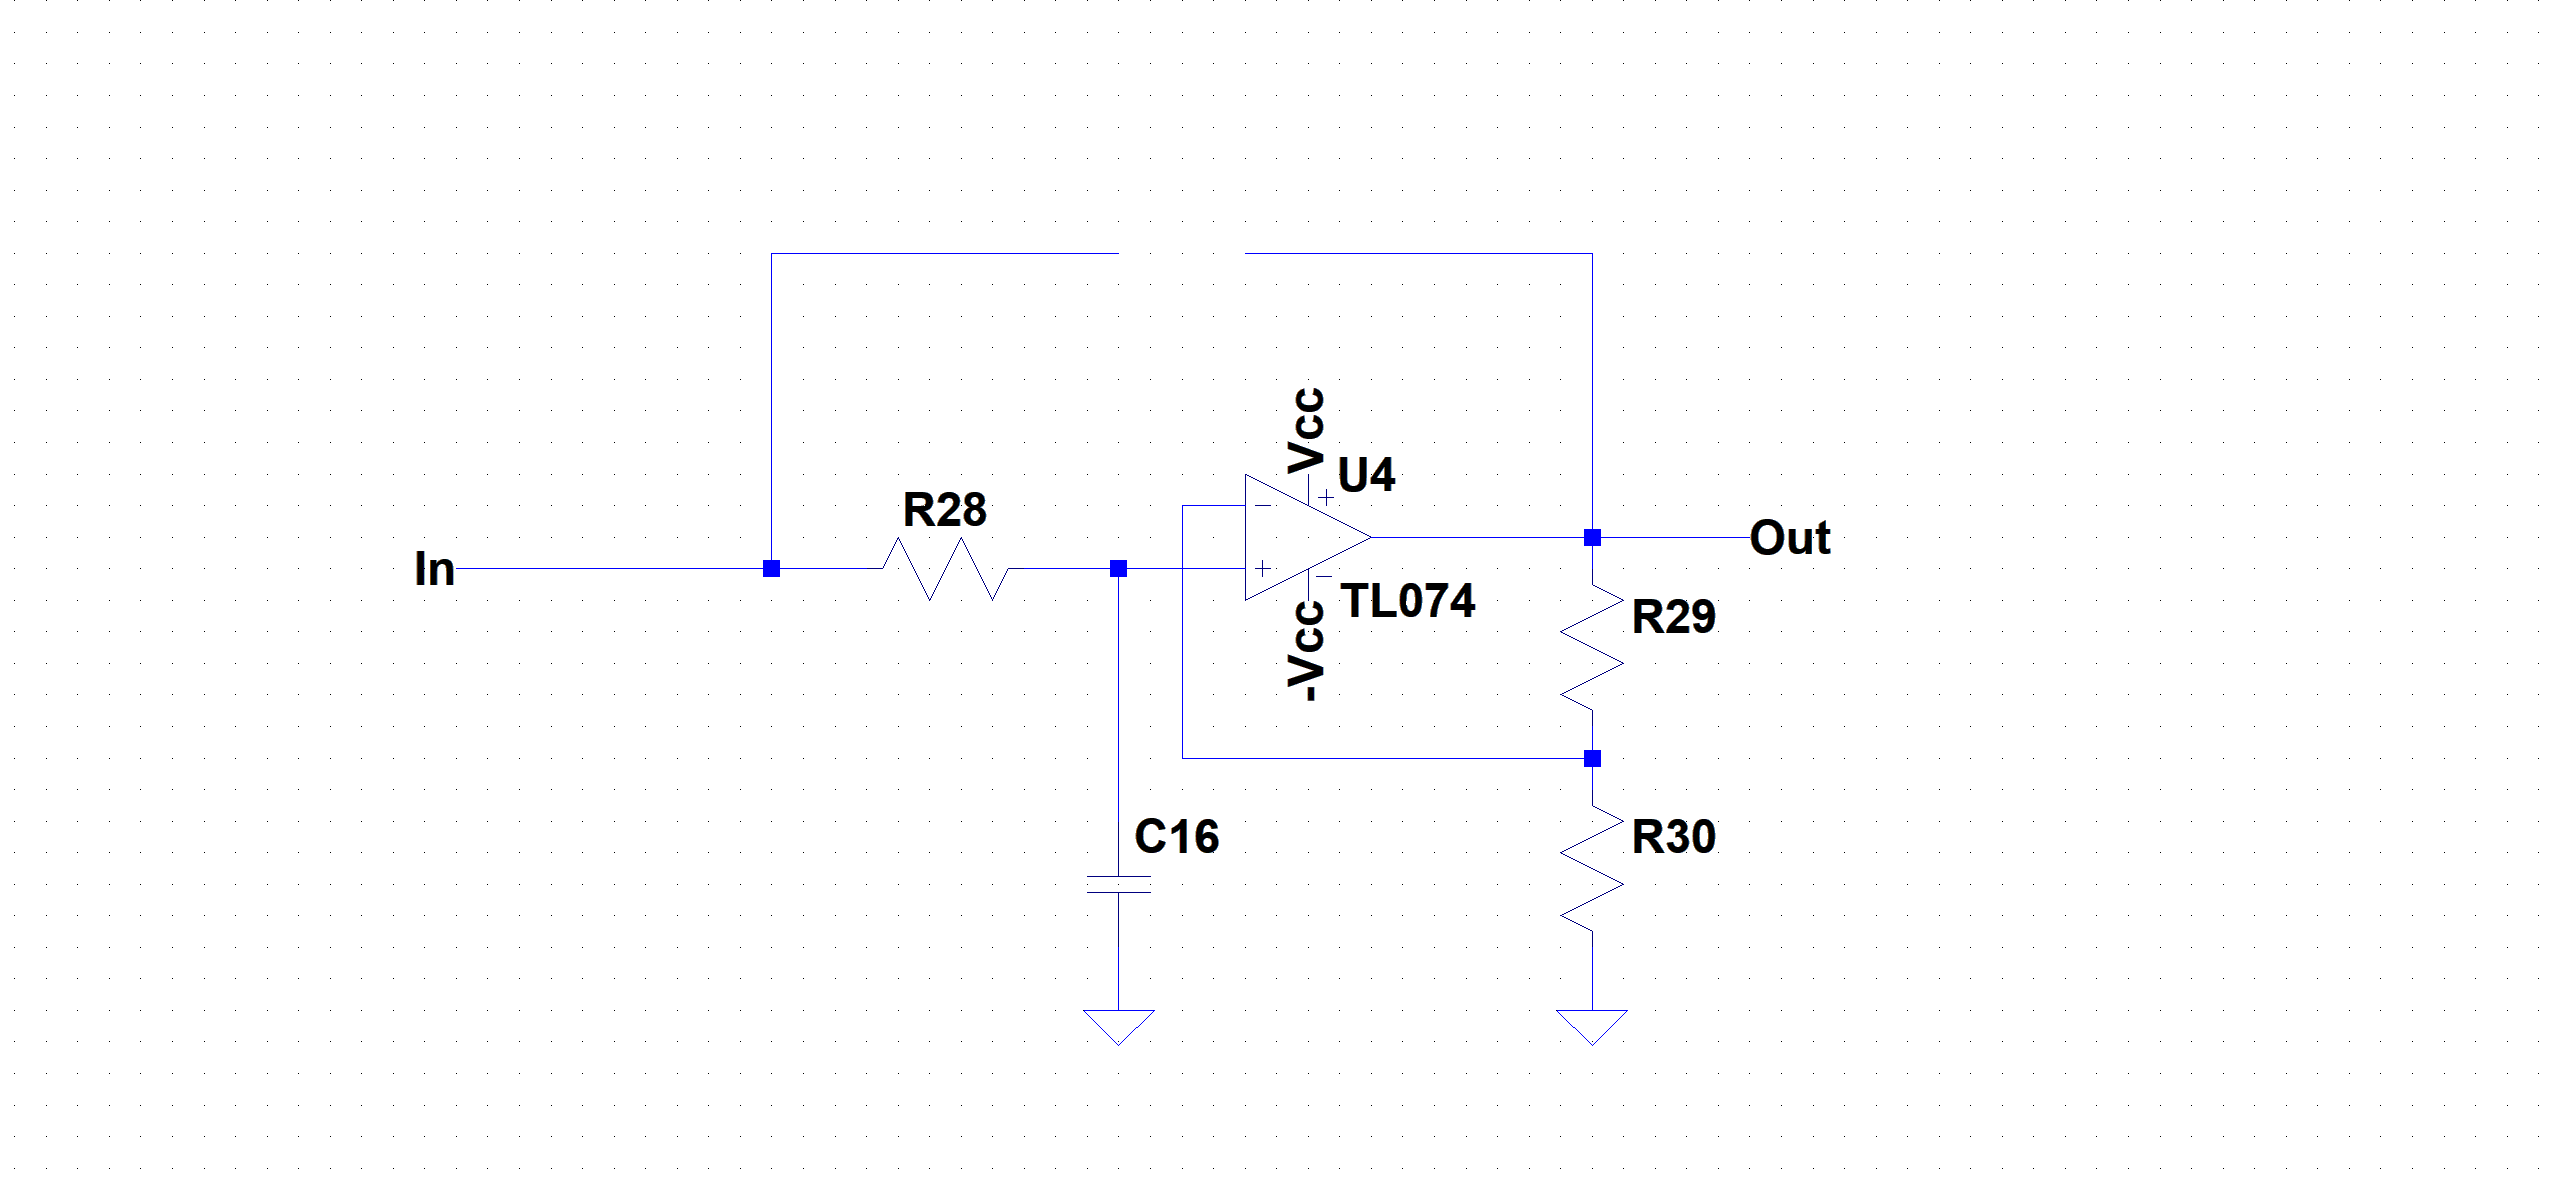
\includegraphics[width=0.9\textwidth]{images/Analoge_Schaltung_Sallentopassive.png}
\caption{Umgebautes Sallen/Key zu passivem Filter 1. Ordnung}
\end{center}
\end{figure}
\end{minipage}

Die Dimensionierung der neuen Schaltung ist mithilfe der nachfolgenden Formel geschehen. Die Verstärkungen konnten beibehalten werden. Die passiven Filter mussten neu berechnet werden.[x]

\begin{minipage}[h]{0.5\textwidth}
\begin{equation}
f_g=\frac{1}{2 \cdot \pi \cdot R_{28} \cdot C_{16}}
\label{eq:Wellenlänge}
\end{equation}

\end{minipage}
\begin{minipage}[h]{0.5\textwidth} 
\begin{equation}
A=1+\frac{R_{29}}{R_{30}}
\label{eq:Wellenlänge}
\end{equation}
\end{minipage}

